\documentclass{standalone}
\usepackage{graphicx}	
\usepackage{amssymb, amsmath}
\usepackage{color}

\usepackage{tikz}
\usetikzlibrary{calc, arrows.meta}
\usepackage{pgfmath}

\definecolor{light}{RGB}{220, 188, 188}
\definecolor{mid}{RGB}{185, 124, 124}
\definecolor{dark}{RGB}{143, 39, 39}
\definecolor{highlight}{RGB}{180, 31, 180}
\definecolor{gray10}{gray}{0.1}
\definecolor{gray20}{gray}{0.2}
\definecolor{gray30}{gray}{0.3}
\definecolor{gray40}{gray}{0.4}
\definecolor{gray60}{gray}{0.6}
\definecolor{gray70}{gray}{0.7}
\definecolor{gray80}{gray}{0.8}
\definecolor{gray90}{gray}{0.9}
\definecolor{gray95}{gray}{0.95}

\newcommand*{\offset}{0.025}

\begin{document}

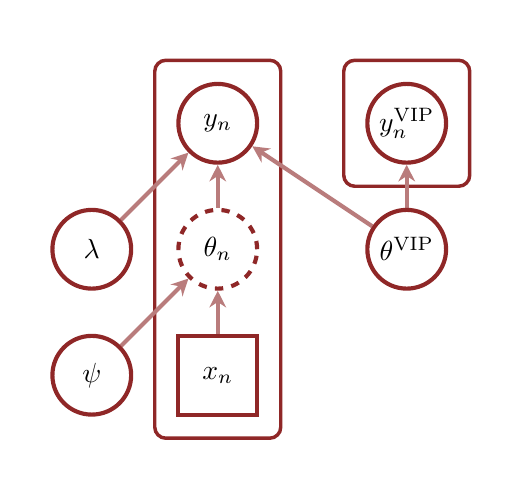
\begin{tikzpicture}[scale=0.2, thick]

  \pgfmathsetmacro{\r}{2.5}
    
  \draw[white] (-12, -6) rectangle (18, 22);

  \coordinate (A) at (0, 0);
  \coordinate (B) at (0, 8);
  \coordinate (C) at (0, 16);
  
  \coordinate (D) at (-8, 0);
  
  \coordinate (E) at (-8, 8);
  \coordinate (F) at (12, 8);
  
  \coordinate (G) at (12, 16);
  
  \draw[dark, line width=1.25, rounded corners=4] (-4, -4) rectangle (4, 20);
  \draw[dark, line width=1.25, rounded corners=4] (8, 12) rectangle (16, 20);

  \foreach \B/\E in {A/B, B/C, D/B, E/C, F/C, F/G} {
    \draw[-{Stealth[length=6pt, width=6pt]}, shorten <=15, shorten >=15, color=mid, line width=1.5] (\B) -- (\E);
  }

  \coordinate (delta) at (\r, \r);
  \filldraw[fill=white, draw=dark, line width=1.5, anchor=center] ($(A) - (delta)$) rectangle ($(A) + (delta)$)
  node[color=black, midway] { $x_{n}$ };

  \filldraw[fill=white, draw=dark, dashed, line width=1.5] (B) circle (\r)
  node[color=black] { $\theta_{n}$ };
  
  \filldraw[fill=white, draw=dark, line width=1.5] (C) circle (\r)
  node[color=black] { $y_{n}$ };
  
  \filldraw[fill=white, draw=dark, line width=1.5] (D) circle (\r)
  node[color=black] { $\psi$ };
  
  \filldraw[fill=white, draw=dark, line width=1.5] (E) circle (\r)
  node[color=black] { $\lambda$ };

  \filldraw[fill=white, draw=dark, line width=1.5] (F) circle (\r)
  node[color=black] { $\theta^{\text{VIP}}$ };
  
  \filldraw[fill=white, draw=dark, line width=1.5] (G) circle (\r)
  node[color=black] { $y^{\text{VIP}}_{n}$ };

\end{tikzpicture}

\end{document}  